\documentclass[9pt,twocolumn,twoside]{pnas-new}

% Use the lineno option to display guide line numbers if required.
% Note that the use of elements such as single-column equations
% may affect the guide line number alignment.
% new commands:

% species names
\newcommand{\cel}{\emph{C.~elegans}}
\newcommand{\dicty}{\emph{D.~discoideum}}
\newcommand{\ecol}{\emph{E.~coli}}

% gene names
\newcommand{\egl}{\emph{egl-9}}
\newcommand{\cysl}{\emph{cysl-1}}
\newcommand{\nog}{\emph{nog-1}}
\newcommand{\rhy}{\emph{rhy-1}}
\newcommand{\vhl}{\emph{vhl-1}}
\newcommand{\eglvhl}{\emph{egl-9;vhl-1}}
\newcommand{\eglhif}{\emph{egl-9;hif-1}}
\newcommand{\hif}{\emph{hif-1}}
\newcommand{\fog}{\emph{fog-2}}
\newcommand{\nhr}{\emph{nhr-57}}
\newcommand{\lam}{\emph{lam-3}}

% protein names
\newcommand{\eglp}{EGL-9}
\newcommand{\rhyp}{RHY-1}
\newcommand{\nogp}{NOG-1}
\newcommand{\vhlp}{VHL-1}
\newcommand{\hifp}{HIF-1}
\newcommand{\fogp}{FOG-2}
\newcommand{\nhrp}{NHR-57}
\newcommand{\lamp}{LAM-3}

% DE genes numbers:
\newcommand{\egln}{1,487}
\newcommand{\rhyn}{1,816}
\newcommand{\vhln}{605}
\newcommand{\eglvhln}{1,989}
\newcommand{\hifn}{481}
\newcommand{\eglhifn}{364}
\newcommand{\fogn}{1,896}
\newcommand{\total}{3,211}
\newcommand{\inall}{53}
\newcommand{\allup}{10}
\newcommand{\alldown}{13}

% downstream targets
\newcommand{\egltargets}{432}
\newcommand{\rhytargets}{1}
\newcommand{\vhltargets}{36}
\newcommand{\hiftargets}{133}

\templatetype{pnasresearcharticle}[9pt,twocolumn,twoside,lineno] % Choose template
% {pnasresearcharticle} = Template for a two-column research article
% {pnasmathematics} = Template for a one-column mathematics article
% {pnasinvited} = Template for a PNAS invited submission

\title{Genetic Analysis of a Metazoan Pathway using Transcriptomic Phenotypes}

% Use letters for affiliations, numbers to show equal authorship (if applicable) and to indicate the corresponding author
% \author[a,b]{David Angeles-Albores}
% \author[a,b]{Carmie Puckett Robinson}
% \author[a]{Brian Williams}
% \author[b]{Igor Antoshechkin}
% \author[a,b]{Paul W Sternberg}
%
% \affil[a]{Department of Biology and Biological Engineering, Caltech, Pasadena, USA, 91125}
% \affil[b]{Howard Hughes Medical Institute}
% \affil[*]{These authors contributed equally to this manuscript}

% Please give the surname of the lead author for the running footer
\leadauthor{Angeles-Albores}

% Please add here a significance statement to explain the relevance of your work
\significancestatement{Measurements of global gene expression are often used as descriptive tools capable of identifying genes that are downstream a perturbation. In theory, there is no reason why measurements of global transcriptomes could not be used as a quantitative phenotype for genetic analysis in multicellular organisms. In fact, qPCR measurements of single or a few reporter genes are already used to perform genetic network analysis. Here, we show that transcriptomes can be used for epistasis analysis in a metazoan, and that transcriptomes afford far more information per experiment than classic genetic analysis. By using transcriptomes as quantitative phenotypes, we can accurately predict interactions between genes, while at the same time identifying genes common to a pathway.
When pathways branch, it is also possible to identify gene batteries that are associated with each end of the branch point. Finally, genes that would result in invisible visible phenotypes in an animal are not likely to be invisible at the transcriptome phenotype due to the exquisite granularity present in these structures, which represents an important advance towards studying small effect genes that make up the majority of animals' genetic repertoire.}

% Please include corresponding author, author contribution and author declaration information
\authorcontributions{DA, CPR and PWS designed the experiments. CPR selected the genes and extracted mRNA from all mutants. BW made the libraries. IA performed all sequencing. DA developed the mathematical theory. DA wrote all computer code and performed all analyses. DA made all the reporter strains and performed all microscopy. DA, CPR and PWS wrote the manuscript.}
\authordeclaration{The authors declare no conflict of interest.}
% \equalauthors{\textsuperscript{1}A.O.(Author One) and A.T. (Author Two) contributed equally to this work (remove if not applicable).}
\correspondingauthor{\textsuperscript{2}To whom correspondence should be addressed. E-mail: pws@caltech.edu}

% Keywords are not mandatory, but authors are strongly encouraged to provide them. If provided, please include two to five keywords, separated by the pipe symbol, e.g:
\keywords{genetics $|$ RNA-Seq $|$ epistasis $|$ hypoxia $|$ transcriptomics $ | $ systems biology}

\begin{abstract}
RNA-Seq is a technology that is commonly used to identify genetic modules that are responsive to a perturbation. In theory, global gene expression could also be used as a phenotype in complex metazoans, with all the implications that has for genetic analysis. To that end, we sequenced the transcriptome of four single mutants and two double mutants of the hypoxia pathway in \cel{}. We successfully analyzed the single mutants in a blinded fashion to predict the genetic relationships between the genes, and used the double mutants as a test of our predictions and to infer the directionality of the relationship.
We show that genes along a pathway tend to decorrelate as a result of alternative regulatory modes and crosstalk with other pathways; and that this decorrelation accurately reflects functional distance between genes. As a by-product of our analysis, we predict \hiftargets{} genes under the regulation of \hif{}, and \vhltargets{} genes under the regulation of \vhl{}. Transcriptomic perturbations suggest an important role of \hif{}-dependent response in chromatin remodelling in \cel{}. Interactive graphics for this paper can be found at \url{www.wormlabcaltech.github.io/mprsq}.\end{abstract}

\dates{This manuscript was compiled on \today}
\doi{\url{www.pnas.org/cgi/doi/10.1073/pnas.XXXXXXXXXX}}

\begin{document}


% Optional adjustment to line up main text (after abstract) of first page with line numbers, when using both lineno and twocolumn options.
% You should only change this length when you've finalised the article contents.
\verticaladjustment{-2pt}

\maketitle
\thispagestyle{firststyle}
\ifthenelse{\boolean{shortarticle}}{\ifthenelse{\boolean{singlecolumn}}{\abscontentformatted}{\abscontent}}{}

% If your first paragraph (i.e. with the \dropcap) contains a list environment (quote, quotation, theorem, definition, enumerate, itemize...), the line after the list may have some extra indentation. If this is the case, add \parshape=0 to the end of the list environment.
\dropcap{G}enetic analysis of molecular pathways has traditionally been performed through epistatic analysis. Epistasis occurs when two genes interact, either directly (biochemical interaction) or through a molecular pathway or physical interaction (genetic interaction). If two genes interact, and the mutants of these genes have a quantifiable phenotype, the double mutant will have a phenotype that is not the sum of the phenotypes of the single mutants that make up its genotype. Epistatic analysis remains a cornerstone of genetics today~\cite{Phillips2008}.

Previous work in \emph{S. cerevisiae} and \dicty{} using microarrays has shown that transcriptomes can be used to infer genetic relationships in simple eukaryotes~\cite{Hughes2000, VanDriessche2005}.
Developments in the area of transcriptomics have brought forward new protocols, such as RNA-Seq~\cite{Mortazavi2008}, and have also made important progress towards cheaper sequencing~\cite{Metzker2010}, better and faster abundance quantification~\cite{Patro2014, Bray2015,Patro2015} and improved differential analysis of gene expression~\cite{Pimentel2016,Trapnell2013}.
As a result, RNA-Seq has been successfully used to identify genetic %key regulatory
modules involved in a variety of processes, including T-cell regulation~\cite{Singer2016,Shalek2013}, the \cel{} linker cell migration~\cite{Schwarz2012}, or planarian stem cell maintenance~\cite{VanWolfswinkel2014,Scimone2014}. However, even in these novel applications, transcriptional profiling largely serves a descriptive role in target gene identification.

To investigate the ability of transcriptomes to serve as quantitative phenotypes, we selected mutants in the \cel{} hypoxia pathway for transcriptome sequencing.
% carmie:
Metazoans depend on the presence of oxygen in sufficient concentrations to  support aerobic metabolism. Genetic pathways evolved to rapidly respond to any acute or chronic changes in oxygen levels at the cellular or organismal level. These oxygen sensitive pathways are involved in a broad range of human pathologies and they have been subject to investigation biochemical and genetic approaches~\cite{Semenza2012}. These approaches identified the Hypoxia Inducible Factors (HIFs) as an important group of oxygen responsive genes.

Hypoxia Inducible Factors are highly conserved in metazoans~\cite{}. A common mechanism for hypoxia-response induction is heterodimerization between a HIF$\alpha$ and a HIF$\beta$ subunit. The heterodimer then initiates transcription of target genes~\cite{}. The number and complexity of HIFs varies throughout metazoans, with humans having three HIF$\alpha$ subunits and two HIF$\beta$ subunits, whereas in the roundworm \emph{Caenorhabditis~elegans} (\cel{}) there is a single HIF$\alpha$ gene, \hif{} and a single HIF$\beta$ gene, \emph{ahr-1}. HIF target genes have been implicated in a wide variety of cellular and extracellular processes such as glycolysis, extracellular matrix modification, autophagy and immunity~\cite{}.

Levels of HIF$\alpha$ proteins tend to be tightly regulated. Under conditions of normoxia, HIF-1$\alpha$ exists in the cytoplasm and partakes in a futile cycle of continuous protein production and rapid degradation with a half-life of minutes~\cite{}. HIF-1$\alpha$ is hydroxylated by three proline hydroxylases in humans (PHD1, PHD2 and PHD3) but is only hydroxylated by one proline hydroxylase (\egl{}) in \cel{}~\cite{}. HIF-1 hydroxylation increases its binding affinity to Von Hippel Lindau Tumor Suppressor 1 (\vhl{}), which allows ubiquitination of HIF-1 leading to its subsequent degradation. In \cel{}, \eglp{} activity is inhibited by binding of CYSL-1, and CYSL-1 activity is in turn inhibited at the protein level by \rhyp{}, possibly by post-translational modifications to CYSL-1~\cite{Ma2012}.
% old:
% The hypoxia pathway is a conserved pathway that is found in all metazoans~\cite{Semenza2012}. It plays an important role in oxygen and iron homeostasis and in the immune response among others~\cite{Nizet2009,Ackerman2012,Kirienko2013}, and it is believed to play an important role in cancer appearance and progression, making it an attractive therapeutic target for disease~\cite{Semenza2003}.
% In \cel{} and other systems, \hifp{} is constitutively degraded by a futile cycle that involves hydroxylation by the EGLN1 ortholog \eglp{}~\cite{,Epstein2001,To2005}, followed by ubiquitination by the von Hippel-Lindau Suppressor 1, \vhlp{}~\cite{Bishop2004,Shao2009,Tanimoto2000,Jaakkola2001}.
% Inhibition of hydroxylation leads to accumulation of activated \hifp{}~\cite{Bishop2004}. Among the known targets of \hifp{} activation are \rhy{} and \egl{}. Increased \rhyp{} activates \eglp{}~\cite{Shen2006,Ma2012}.

Here, we show that transcriptomes contain strong, robust signals that can be used to infer relationships between genes in complex metazoans by reconstructing a the hypoxia pathway in \cel{} using RNA-Seq. To reconstruct this pathway, we developed new analytic mathematical tools to query genetic interactions at the transcriptome level. We used these analytic tools to generate a method for analyzing transcriptome genetics data, which we termed Metazoan RNA-based Gene Analysis (MoRGAn).
% Our goal is not to generate a high-quality database of hypoxia-related genes, but rather to perform a quantitative genetic analysis analogous to classical genetics.
% Using MoRGAn, we show that various techniques, including pairwise transcriptome comparisons, expression clustering or \emph{in silico} qPCR can be used to generate a testable model of genetic interactions.
We show that MoRGAn provides a sound theoretical and experimental framework with which to dissect genetic pathways. Using MoRGAn, we were able to reconstruct interactions between genes in the hypoxia pathway.
Furthermore, we show that the phenomenon of phenotypic epistasis, a hallmark of genetic interaction, holds at the molecular systems level.
We also demonstrate that transcriptomes contain sufficient information, under certain circumstances, to order genes in a pathway using only single mutants. Finally, we were able to identify genes that appear to be downstream of \egl{} and \vhl{}, but are almost certainly not targets of \hif{}.
A complete, interactive version of the analysis is also available at \url{www.wormlabcaltech.github.io/mprsq}.

\section*{Results}
\subsection{Development of a New Genetic Logic for Vectorial Phenotypes}
\label{sec:genetic_logic}

Transcriptomes can be understood as information-rich phenotypes that are fine-grained representations of an organism's internal state (citation?)~\cite{}. As transcriptomes have become more prominent, the single-cell community in particualr has begun to use them to define and understand cellular identities~\cite{}. However, most approaches rely on data-driven, computational methods to define the important or relevant aspects of a transcriptomes and the community is actively developing new algorithms for increasingly complex data. On the other hand, whole-organism transcriptomes have not been analyzed quite so exhaustively, partially because these transcriptomes contain the identities of multiple cell-types in one convoluted measurement.

Although computational advances for RNA-seq analysis are important, an equally important facet of transcriptome analysis is the development of analytical mathematical tools with which to understand these objects. In an effort to understand transcriptome genetics at a profound level, we developed extensions to standard genetic theory borrowing from concepts in group and operator theory that enabled us to think logically about genetics using a vectorial phenotype.

Briefly, we envisioned that a single gene is always associated with the same specific transcriptome under a set of specified conditions (age of the organism, ambient temperature, food status, etc\dots). We refer to the set of genes that are differentially expressed in response to a perturbation of a gene as a specific transcriptome. A specific transcriptome can be formally thought of as a group of genes with an associated metric for each gene (such as abundance, fold change or log-fold change), or equivalently as a function that takes as input a gene ID and outputs a scalar.
However, although a global transcriptome is fundamentally an observable quantity, the specific transcriptome associated with a gene is not, since we do not know the identities of the genes that incorporate it. In order to observe a specific transcriptome, it is necessary to perform at least two experiments: first, we must measure a basal transcriptome; second, we must measure a transcriptome in a set of organisms that have a perturbed activity of the gene in question.

Having established the concept of a specific transcriptome as a group of ordered tuples of the form (gene, measurement), we reasoned that transcriptomes should obey the laws of genetic networks. Namely, we reasoned that if two hypothetical genes, $A$ and $B$, act in a linear unbranched pathway, then $A$ and $B$ should have equivalent specific transcriptomes. We also reasoned that if $A$ acts upon two different pathways, one which involves B and one which doesn't, the specific transcriptome of $A$ should itself be separable into two independent parts: the specific transcriptome associated with the pathway $A\rightarrow B$, and the specific transcriptome associated with $A$ but not $B$.

In order to solve genetic pathways, it is not sufficient to measure two transcriptomes and compare the overlap between the genes they contain. To solve complex genetic pathways, we must understand the valence of a genetic interaction between genes. In order to do this, we created linear operators to model perturbations that increase or decrease the activity of a gene relative to the basal measured state. These linear operators allow us to propagate a perturbation in one gene through a network and predict the expected changes in specific transcriptomes associated with the other genes in a network subject to the genetic model that has been specified by the investigator.

Using this formalism, we are, in theory, able to infer genetic relationships between genes. However, this formalism also provides a rational framework with which to identify specific transcriptomes associated with a pathway, and it also provides a theoretical manner with which to order genes acting along a pathway if the pathway branches at multiple points. Finally, our methods can allow us to identify regulatory relationships that are acting on different levels (either at the transcriptional level or at the protein level).
For example, assuming that the mode of interaction between \rhy{} and \egl{} is the same as the mode of interaction between \hif{} and \rhy{} (transcriptional control) leads to aberrant behavior that is not observed empirically. Only by assuming that the regulatory mode between \rhy{} and \egl{} is different than between \hif{} and \rhy{} does the model generate predictions that parallel reality. Our new genetic notation, and the concepts contained therein, represent an important advance towards harnessing the power of transcriptomes as quantitative phenotypes. For a full description of this notation, see the S.I..

\subsection{Clustering visualizes epistatic relationships between genes}
\label{sub:Clustering}

As a first step in our analysis, we analyzed our data using a generalized linear model with a genotype term (see~\ref{methods}) on logarithm-transformed counts. Genes that are significantly altered between wild-type and a given mutant have a genotype coefficient that is statistically significantly different from 0. We refer to these coefficients through the greek letter $\beta$. These coefficients are not identical to the average log-fold change per gene, although they are loosely related to this quantity. In general, larger $\beta$ magnitudes correspond to larger perturbations. These coefficients can be used to study the RNA-Seq data in question.

Clustering is a well-known technique in bioinformatics that is used to identify relationships between high dimensional data points~\cite{Yeung2003}. We wanted to make sure that clustering by differential expression yielded genetically relevant information. \hif{} exhibits no obvious phenotypes under normoxic conditions, in contrast to \egl{}, which exhibits an egg-laying (\emph{egl}) phenotype in the same environment. \egl{}; \hif{} mutants suppress the \emph{egl} phenotype. If transcriptomic phenotypes behave similarly to their macroscopic counterparts, \hif{} should cluster with the \egl{}; \hif{} double mutant, whereas \egl{} should cluster away from the \hif{} mutant.
Indeed, when blind, unsupervised clustering was performed on the data, three clusters emerged. \hif{} and \egl{};\hif{} clustered together, indicating suppression of the \egl{} phenotype; whereas \egl{}, \egl{};\vhl{}, \vhl{} and \rhy{} all clustered separately. Finally, our negative control \fog{} was in its own cluster (see Fig.~\ref{fig:dendrogram}). We conclude that expression data contains enough signal to cluster genes in a meaningful manner in complex metazoans.

% dendrogram
\begin{figure}%[tbhp]
\centering
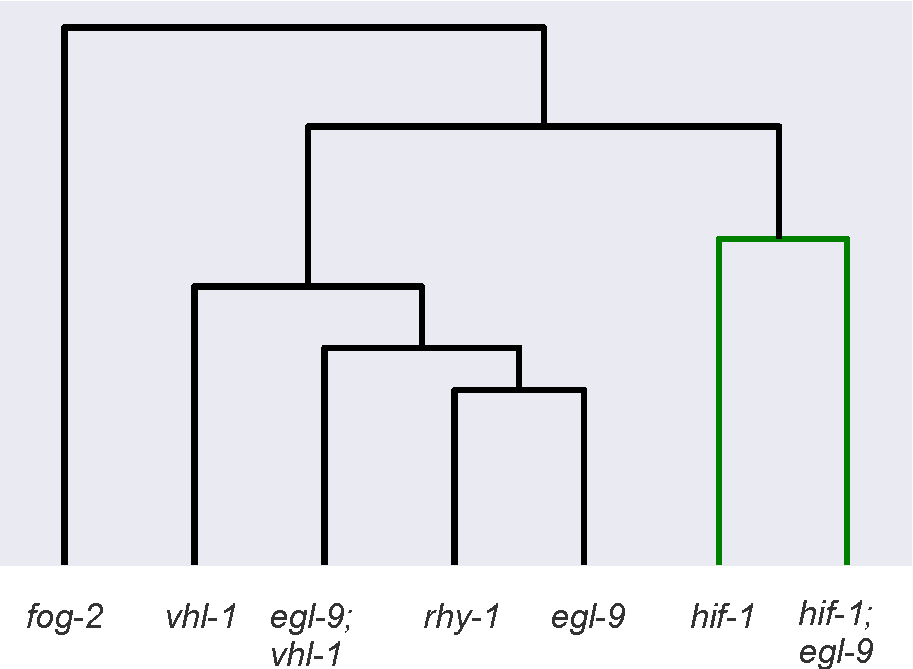
\includegraphics[width=\linewidth]{figs/dendrogram.pdf}
\caption{Blind unsupervised clustering of various \cel{} mutants. Genes cluster in a manner that is biologically intuitive. Genes that inhibit \hif{} (i.e, \egl{}, \vhl{}, and \rhy{}) cluster far from \hif{}. \hif{} clusters with the suppressed \egl{}; \hif{} double mutant. A control gene, \fog{}, clusters farthest away.}
\label{fig:dendrogram}
\end{figure}

\subsection{Transcriptomic correlations can predict genetic regulation}
\label{sub:Transcriptomic genetic analyses}

% TODO: Add SI link at end of paragraph.
Theoretically, two genes that share linear positive regulation should be positively correlated in their overlapping transcriptomes, whereas two genes that share linear negative regulation should be negatively correlated in their transcriptomes.
% Formally, if we consider that a gene \emph{A} has a transcriptome \emph{\{A\}} associated with it, and if we consider a second gene \emph{B} with an associated transcriptome \emph{\{B\}} that is activated by \emph{A} (that is, $B \in \{A\}$, such that $\{B\} \subset \{A\}$), then it follows that genetic knockout of \emph{A} or \emph{B} should both lead to the same perturbation of the transcriptome \emph{\{B\}}.
Conversely, it follows that if two mutants have overlapping transcriptomes that are strongly positively correlated, it is likely that these two genes share a positive regulatory association. In other words, transcriptomic correlation is a good predictor of genetic regulation. For a formal introduction to the genetic logic, see S.I..

Although transcriptomic correlations could theoretically be used for the purposes of identifying genetic regulation, noise can cause serious interference with any inferences. Additionally, genes sometimes experience multiple modes of regulation, including positive and negative regulation, from the same gene or pathway. Because we are measuring the system at steady state, both modes of regulation will be measured simultaneously. If a positive and a negative signal of equal strength are both present in a transcriptome, running a naive regression may result in a value close to zero.
Therefore, we took steps to mitigate noise emanating from frequent outliers and to identify multiple regulatory signals.

To mitigate noise, we rank-tranformed the $\beta$ coefficients for each mutant. This has the effect of mitigating outliers by resetting the difference between adjacent coefficients to unity. Next, we performed robust Bayesian regressions using a Student-T distribution as a prior. A Student-T distribution decays less quickly than a normal distribution, which causes the model to consider outliers to be less informative than traditional regressions.

% genetic correlations
\begin{figure}%[tbhp]
\centering
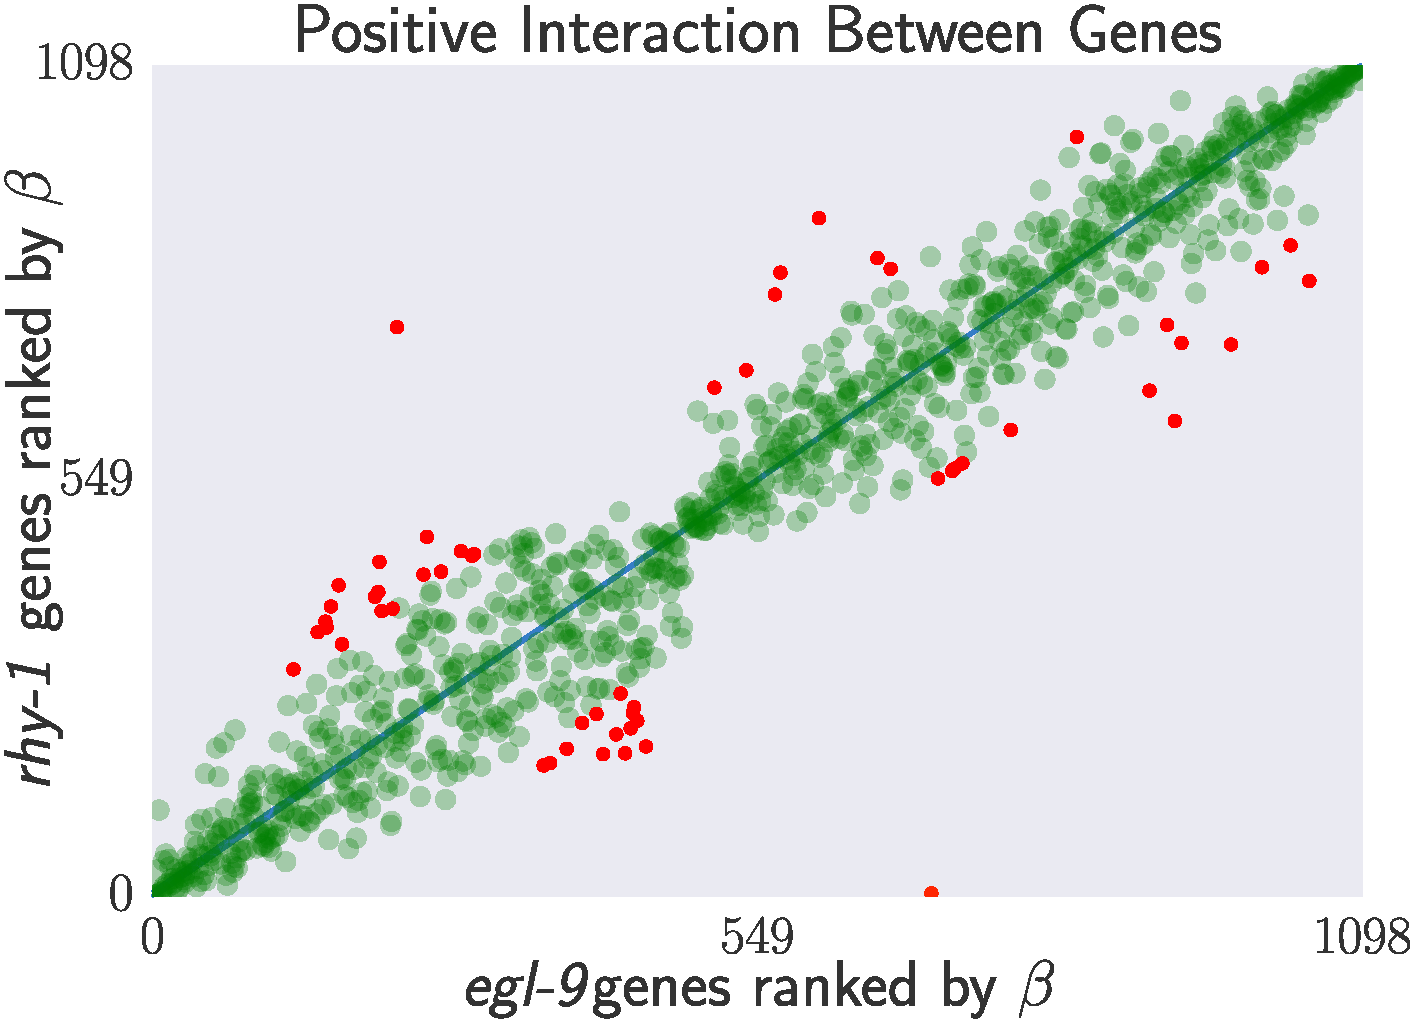
\includegraphics[width=\linewidth]{figs/correlative_genetics.pdf}
\caption{Strong transcriptional correlations can be identified between genes that share a positive regulatory connection. We took the \egl{} and the \rhy{} transcriptomes, identified differentially expressed genes common to both transcriptomes and ranked each gene according to its differential expression coefficient $\beta$. We then plotted the rank of each gene in \rhy{} versus the rank of the same gene in the \egl{} transcriptome. The result is an almost perfect correlation. For unknown genes, such a correlation would be predictive of an interaction.}
\label{fig:genetic_interactions}
\end{figure}

% TODO: Check if egl was in fact first identified as a hif target
% TODO: SI links
We saw that certain gene pairs correlated very well when genes were ranked by their expression changes (see Fig.~\ref{fig:genetic_interactions}). We generated all pairwise correlations between transcriptomes and we weighted the correlations by the number of genes that participated in the correlation (that were not outliers) divided by the total number of genes detected in all samples.
We were able to identify a strong positive interaction between \egl{} and \rhy{}. The transcriptomes for these genes consisted of \egln{} and \rhyn{} significantly altered genes respectively and the overlap between both transcriptomes was extensive. On the other hand, none of the primary correlations between \hif{} and its controlling genes were negative. We were unable to definitively determine the reason for behind this. The overlap between \hif{} and all other genes was relatively small, and each overlap involved different sets of genes, which suggests that we did not sequence deeply enough to identify the nature of these positive interactions. See SI A for an exhaustive analysis of the expected and observed correlation between each gene pair in this circuit respectively.
The regression slopes recapitulated a network with three `modules': A control module, a responder module and an uncorrelated module (see Fig.~\ref{fig:heatmap}). We were able to identify a strong positive interaction between \egl{} and \rhy{}. The magnitude of this weighted correlation is derived from the fact that the transcriptomes for these genes consisted of \egln{} and \rhyn{} significantly altered genes respectively and the overlap between both genes was quite extensive, which makes the weighting factor considerably larger than other pairs.
% On the other hand, none of the primary correlations between \hif{} and its controlling genes are negative. We suspect that this is a result of the profound control that \hif{} exerts on \egl{} and \rhy{}. See SI A and B for an exhaustive analysis of the expected and observed correlation between each gene pair in this circuit respectively.
% heatmap
\begin{figure}[tbhp]
\centering
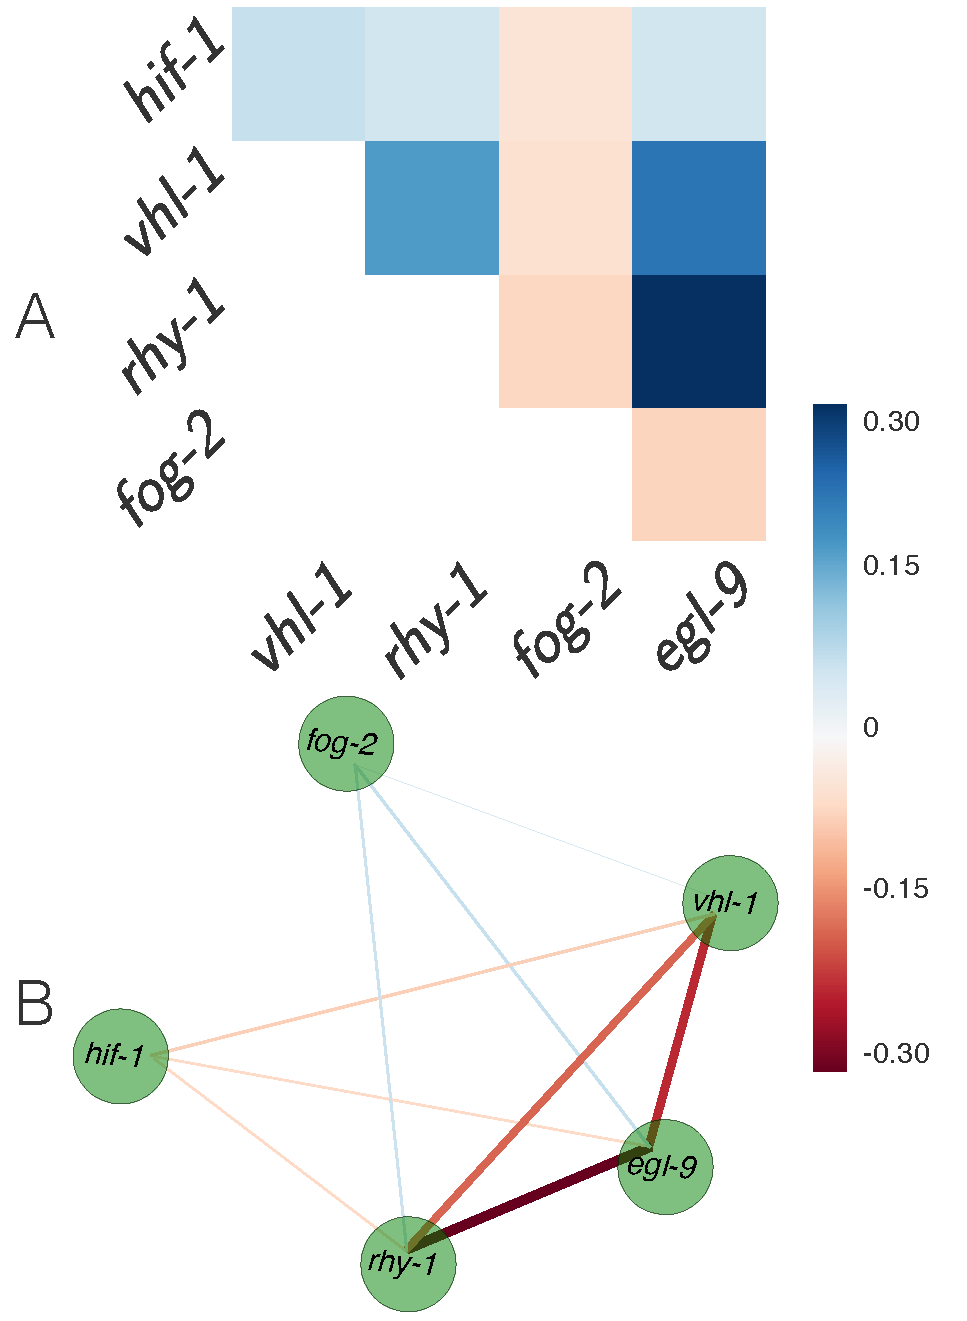
\includegraphics[width=\linewidth]{figs/bayesian_heat_map.pdf}
\caption{\textbf{Top}: Heatmap showing pairwise regression values between all single mutants. \textbf{Bottom}: Correlation network drawn from the diagram. Edge width is proportional to the weighted correlation between two nodes raised to the power of 1.15. % TODO: CHECK
Making the edge width proportional to a power of the regression makes differences in the weighted correlations easier to see.}
\label{fig:heatmap}
\end{figure}

Previous work in the hypoxia pathway has found extensive feedback loops in this pathway. Using the genetic formalism we developed, we realized that due to the fine-grained nature of interactomes we can use them to measure two regulatory interactions of opposite sign simultaneously in a single gene pair.
% Consider a system in which an arbitrary gene A activates a gene B, which in turn blocks a gene C. Each gene X has a specific transcriptome \emph{\{X\}}.Under this system, B and C should have transcriptomes that are negatively correlated. If C activates A, then knocking out B should augment expression of C, which should in turn increase expression of A.
% However, knocking out C should lead to less A, which in turn will lead to less B. Under this thought experiment, suppose that we know the specific transcriptomes associated with A, B and C:\@\emph{\{A\}}, \emph{\{B\}}, \emph{\{C\}}. Then it must be the case that the genetic knockout of B must have a perturbed transcriptomes $\{A^2\}, \{B^0\}, \{C^2\}$. On the other hand, knocking out C must lead to the perturbed transcriptomes $\{A^0\}, \{B^0\}, \{C^0\}$.
% Now, if we were able to correlate each specific transcriptome between correlations, we would find that the specific transcriptomes associated with A and C are anti-correlated; whereas the specific transcriptome associated with B is correlated between both genotypes.
This should lead to a characteristic \emph{X} pattern in the ranked data. Such cross patterns can be indicative of feedback loops or of incoherent regulation at two distinct levels of gene expression (see Fig~\ref{fig:xpattern}). For any gene that has a \emph{X}-patterned diagram, we refer to the correlation that contains the largest number of participating isoforms as the primary correlation, and the correlation that contains the lesser number of points is referred to as a secondary correlation. In our dataset, all primary correlations were positive.

% correlative genetics again
\begin{figure}[tbhp]
\centering
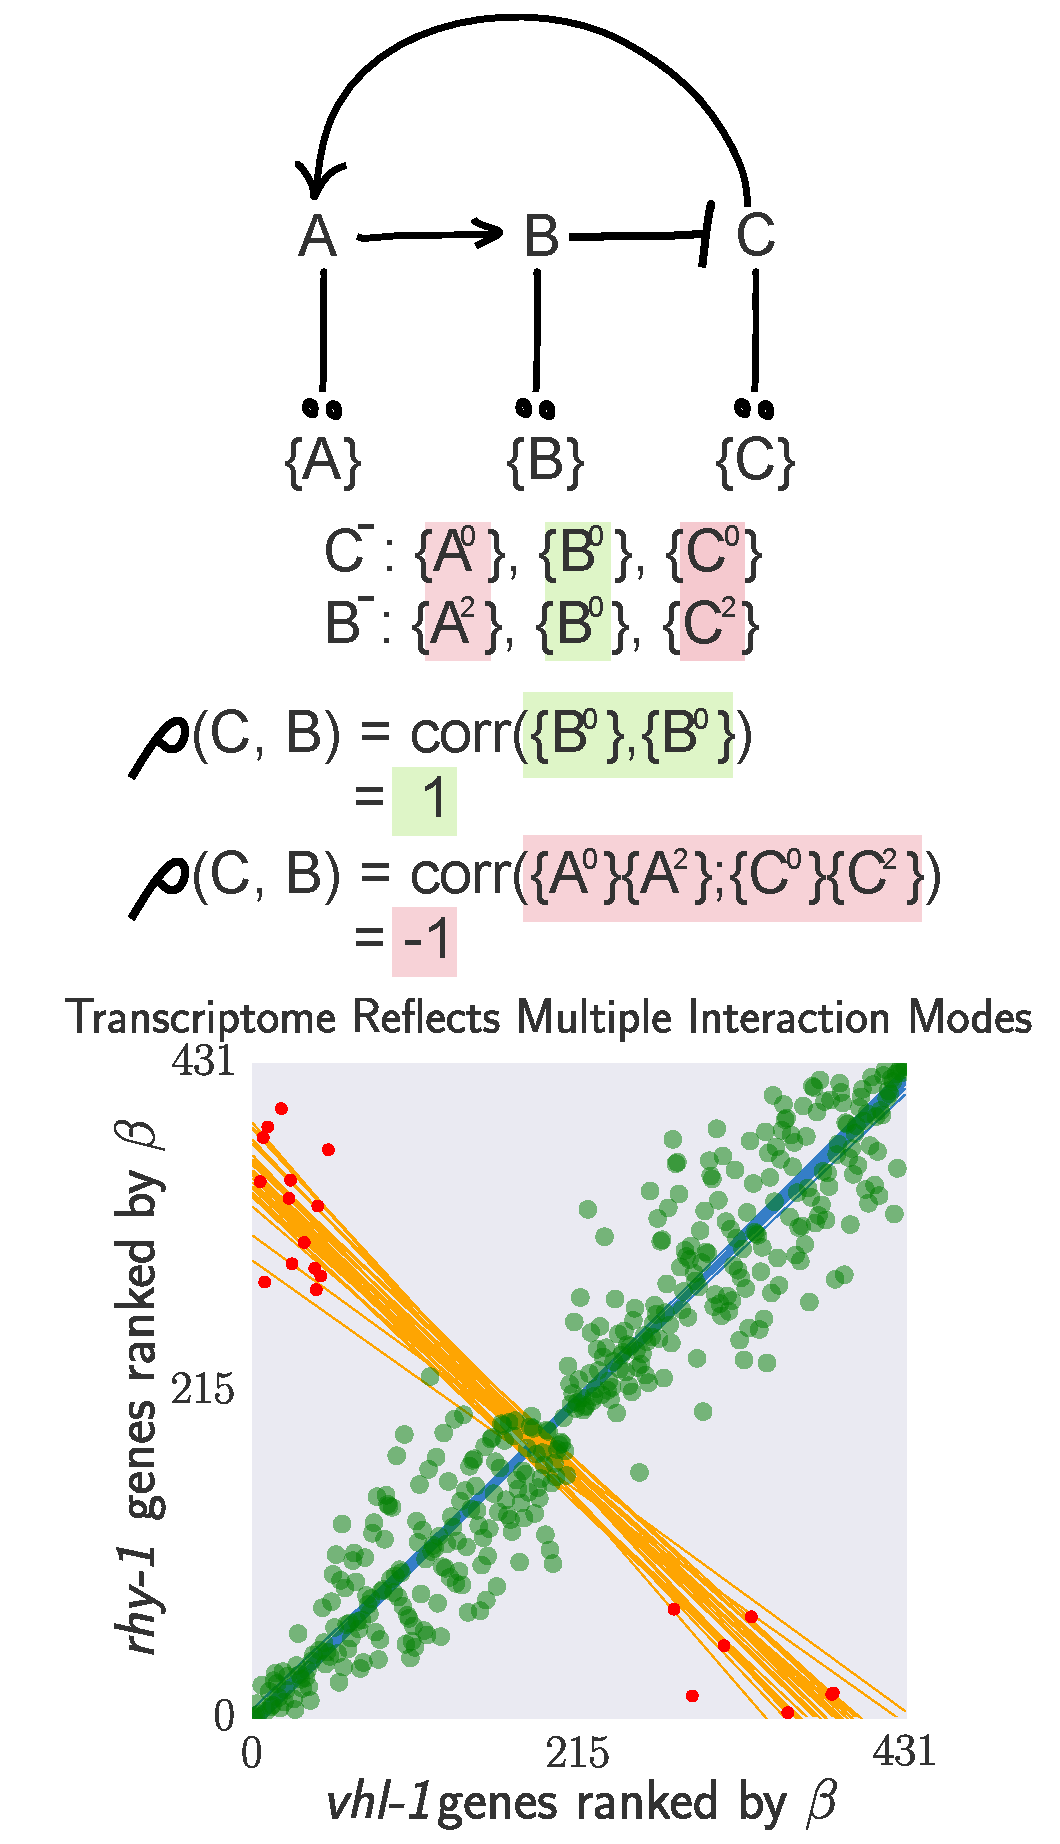
\includegraphics[width=\linewidth]{figs/correlative_genetics2.pdf}
\caption{\textbf{Top}: A feedback loop can generate transcriptomes that are both correlated and anti-correlated. \textbf{Bottom}: \hif{} transcriptome correlated to the \rhy{} transcriptome. Green large points are inliers to the first regression. Red small points are outliers to the first regression. Only the red small points were used for the secondary regression. Blue lines are representative samples of the primary bootstrapped regression lines. Orange lines are representative samples of the secondary bootstrapped regression lines.}
\label{fig:xpattern}
\end{figure}

% TODO SI link
% We investigated whether any pairwise comparisons between our single mutants generated this cross pattern. Indeed, we found that comparing \hif{} with \rhy{}, and \hif{} with \egl{} yielded negative correlations, as did \rhy{} and \vhl{}. While the number of genes that lead these negative correlations is not significant as assessed by a hypergeometric test, these outliers are expected for this circuit (see SI). Statistical information should be integrated holistically with genetic models to assess whether outliers are meaningful or not. Since \hif{} was off in the conditions under which we performed our experiment, measurement of the \hif{} transcriptome is difficult and we suspect the small number of outliers is the result of this low resolution.
We investigated whether any pairwise comparisons between our single mutants generated this cross pattern. Indeed, we found that comparing \hif{} with \rhy{}, and \hif{} with \egl{} yielded negative correlations, as did \rhy{} and \vhl{}. While the number of genes that lead these negative correlations is small (10--30 genes in any comparison) and is not significantly different from random expectation as assessed by a hypergeometric test, these outliers are expected for this circuit (see SI). On the other hand, unweighted secondary correlations had coefficients near unity for most comparisons, and they are predicted by theory. Statistical information should be integrated holistically with genetic models to assess whether outliers are meaningful or not. In our case, we believe that these outliers reflect meaningful interactions between genes in the hypoxia circuit, not random noise.


\subsection{\emph{in silico} qPCR reveals extensive feedback in the hypoxia pathway}
\label{sub:qPCR}
Our dataset enables us to perform a sort of \emph{in silico} qPCR by selectively looking at expression of a few genes at a time. To verify the quality of our data, we queried the changes in expression of \nhr{}. This reporter has been shown to have \hif{} dependent expression~\cite{Shen2006,Shen2005,Ackerman2012,Park2012}. In our dataset, this gene be upregulated in \egl{}, \rhy{} and \vhl{}, but remains unchanged in \hif{}.
The \egl{};\vhl{} had an expression level similar to \egl{}; whereas the \egl{};\hif{} mutant showed suppression of the reporter expression. All of these interactions reflect the literature.

% in silico qPCR
\begin{figure}[tbhp]
\centering
\includegraphics[width=\linewidth]{figs/qpcr.pdf}
\caption{\textbf{Top}: \emph{In silico} qPCR results. \nhr{} is an expression reporter that has been used previously to identify \hif{} regulators~\cite{Shen2006,Shao2009}. The \nhr{} mRNA levels replicate what is observed in the literature. \lam{} is shown here as a negative control that should not be altered by mutations in this pathway. The increases in the levels of \egl{} and \rhy{} when repressors of \hif{} are knocked out are in agreement with previous literature~\cite{Powell-Coffman2010}. We measured modest increases in the levels of \rhy{} mRNA when \hif{} is knocked out. The mechanism behind this is unclear. Negative and positive feedback loops from \hif{} into its inhibiting genes could be a homeostatic mechanism.}
\label{fig:qpcr}
\end{figure}

We also performed \emph{in silico} qPCR of every gene under scrutiny to get a clearer idea of the relationships between them (see Fig.~\ref{fig:qpcr}). We observed changes in \rhy{} expression consistent with previous literature~\cite{} when \hif{} is activated. We also observed changes in \egl{} expression when \egl{} was mutated, and previous literature has identified \egl{} as a hypoxia responsive gene~\cite{}. Although \egl{} was not increased in \rhy{} and \vhl{} mutants, the mRNA levels of \egl{} trended towards increased expression.
As with \nhr{}, the \egl{} and \rhy{} expression phenotypes were abrogated in the \egl{};\hif{} mutant; whereas the \egl{};\vhl{} mutant showed expression phenotypes identical to the \egl{} mutant, in support of \egl{} and \vhl{} acting in an AND-gated manner.
% We found that \rhy{} transcription levels were increased by mutations in \egl{}, \rhy{} and \vhl{}. This suggests that \hif{} is a positive regulator of \rhy{}.
% \egl{} was upregulated in response to mutations in \egl{}. Although the increases were not statistically significant, \rhy{} and \vhl{} also showed trends towards increasing levels of \egl{} expression. The \egl{};\vhl{} double mutant exhibited similar levels of mRNA expression to the \egl{} mutant. On the other hand, the \egl{};\hif{} mutant had wild-type expression of \egl{}. These observations would be sufficient to establish \egl{} as an inhibitor of \hif{}, and to establish \hif{} as a regulator of \egl{}.
Our dataset also shows that knockout of \hif{} resulted in a modest increase in the levels of \rhy{}. This suggests that \hif{} is also a negative regulator of \rhy{}.
% One potential mechanism through which \hif{} could be both a positive and a negative regulator would be for \hifp{} to change its activity when it gets hydroxylated. Under this mechanism, loss of hydroxylated \hifp{} leads to activation of \rhy{} and \egl{} as a homeostatic mechanism, whereas excessive hydroxylation causes inhibition of these genes.

% Given that \rhy{} post-translationally controls \egl{}~\cite{Ma2012}, it is unlikely that the increase in \egl{} is driven by the increase in \rhy{} levels. Therefore, our experiment also suggests that \hif{} is a positive regulator of \egl{}. On the other hand, we also discovered that mutation of \hif{} increased levels of \rhy{}. This suggests that \hif{} is also a negative regulator of \rhy{}. One potential mechanism through which \hif{} could be both a positive and a negative regulator would be for hydroxylation of \hifp{} to change its activity. Under this mechanism, loss of hydroxylated \hifp{} leads to activation of \rhy{} and \egl{} as a homeostatic mechanism, whereas excessive hydroxylation causes inhibition of these genes.

% Whereas loss of hydroxylation seems to lead to overexpression of \rhy{} and \egl{}, there is no change in \hif{} levels. The only change in expression level of this gene occurs in the \hif{} mutant\footnote{We cannot discard the possibility that this decrease in mRNA levels is not due to NMD or some other decay mechanism, but we consider such a large change unlikely}. Therefore, we postulate that \hifp{} positively autoregulates itself only in its hydroxylated state.

% Performing the \emph{in silico} experiment with the \egl{};\vhl{} double mutant shows a very similar $\beta$ coefficient to the \egl{} mutant and suggests that \egl{} and \vhl{} are epistatic to one another. Such epistasis can only occur in one of two ways: Either the genes are acting linearly, or they are acting in AND gated fashion, with both genes required to mediate an effect. Similarly, the \egl{};\hif{} double mutant exhibits the same expression profile as \hif{}, which means \egl{} is an inhibitor of \hif{}.

In summary, the \emph{in silico} qPCR results recapitulate previous results that show \egl{} and \vhl{} act in concert to inhibit \hif{}. Moreover, these results taken together with the transcriptome-wide cross-patterns that emerge from pairwise comparisons between genes in the hypoxia pathway suggest that there are both positive and negative feedback loops feeding into \rhy{} and possibly \egl{}. These feedback loops could explain why \hif{} is positively transcriptomically correlated with \egl{}.

\subsection{Epistasis effects can be detected and quantified.}
\label{sub:Epistasis}
To quantify any epistasis between \egl{} and \vhl{} in our dataset, we identified the genes that were shared between each single mutant and the double mutant \egl{};\vhl{}. If two genes act, for example, in a linear manner, then the double mutant should exhibit an identical phenotype to each single mutant. To test such a relationship, we can plot the difference in a gene $i$ between the log change in expression between the two mutants, $\Delta_i = \beta_{\mathrm{Double~Mutant}, i} - \beta_{\mathrm{Single~Mutant}, i}$, against the log change in the single mutant,  $\beta_{\mathrm{Single~Mutant}, i}$. We can then fit a weighted linear regression to measure the slope of best fit. Genes that act in a linear pathway should yield lines with a slope of 0. Genes that have some additive flavor should have slopes greater than 0. Suppression, a hallmark of inhibition, should yield a slope less than 0.

We observe that the \egl{};\vhl{} mutant has an identical phenotype to the \egl{} single mutant (slope = 0; see Table.~\ref{tab:double_mutant_comparison}). On the other hand, \vhl{} has a positive slope, indicating that \egl{} is additive to \vhl{}. Such partial additivity can be explained if \egl{} is inhibiting \hif{} in a \vhl{}-dependent as well as a \vhl{}-independent manner~\cite{Shao2009}.

% double mutant analysis
\begin{table}%[tbhp]
\centering
\caption{Response Modeling of Double Mutants to Single Mutants}
\begin{tabular}{llrrr}
Double Mutant & Single Mutant & $\Delta$ & SE & p-value\\
\midrule
1. \egl{};\vhl{} & \egl{} & $0.00$ & $0.01$ & $0.81$\\
2. \egl{};\vhl{} & \vhl{} & $0.28$ & $0.033$ & $10^{-15}$\\
3. \egl{};\hif{} & \egl{} & $-0.85$ & $0.074$ & $10^{-13}$\\
4. \egl{};\hif{} & \hif{} & $-0.18$ & $0.10$ & $0.10$\\
\bottomrule
\end{tabular}

\addtabletext{Table showing changes between single and double mutants. $\Delta$ is the result of a weighted-linear regression (WLS) between $\beta_\mathrm{Single~Mutant}$ and $\Delta = \beta_\mathrm{Double~Mutant} - \beta_\mathrm{Single~Mutant}$. $\Delta$ > 0 represents a more severe phenotype than the single mutant. $\Delta$ < 0 represents a suppressed phenotype relative to the single mutant. $\Delta$ = 0 is expected for linear pathways or genes that are acting in linear or AND-gated fashion. $\Delta > 0$ is expected for genes that are acting additively on a pathway. WLS were performed only on genes that were significantly altered in both single mutants and the double mutant. $1+\Delta$ is a very close approximation to the line of best fit between single mutant and double mutant.}
\label{tab:double_mutant_comparison}
\end{table}

% epistasis graph
\begin{figure}[tbhp]
\centering
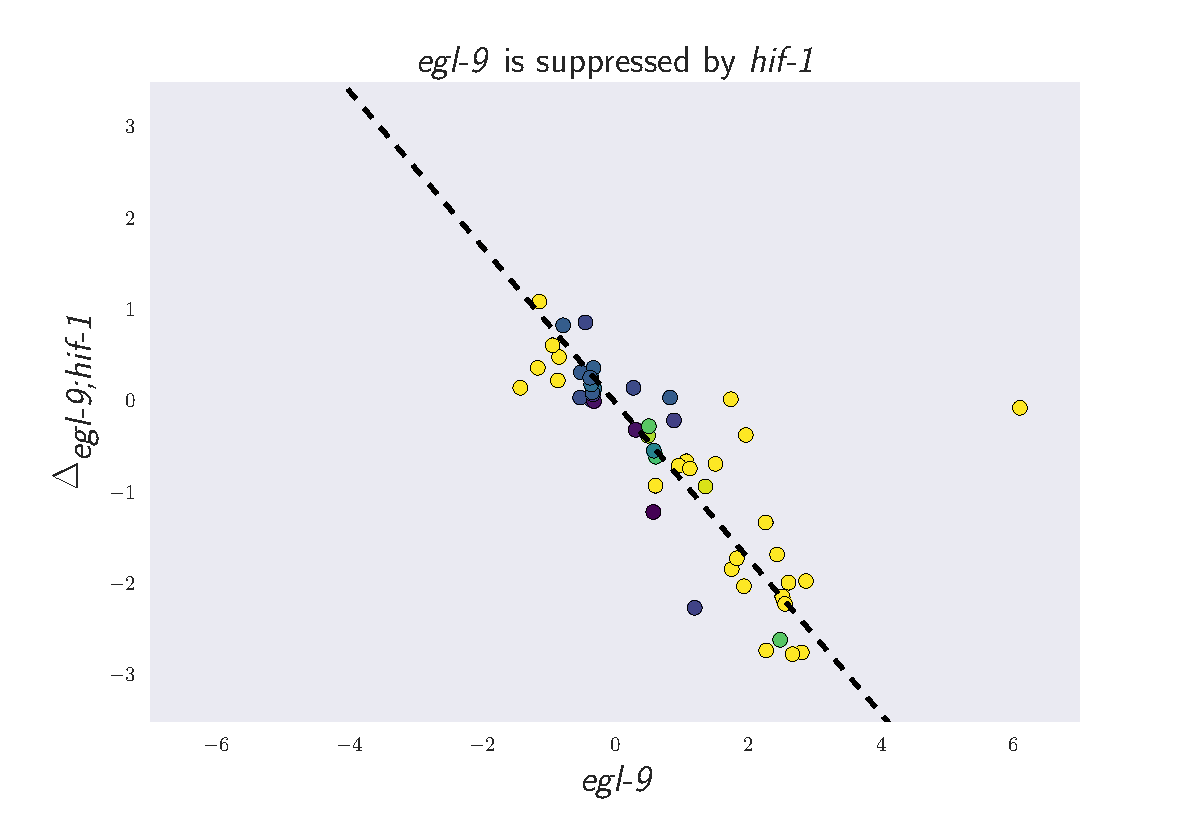
\includegraphics[width=\linewidth]{figs/egl9_epistatic_eglhif.pdf}
\caption{
The mutant \egl{} transcriptomic phenotype is suppressed by mutations in \hif{}. The graph shows the $\beta$ coefficients for \egl{} in the x-axis, and the change in $\beta$ coefficient between the \egl;\hif{} and \egl{} mutant. The dotted line is the regression line between the complete \egl{} and \egl{};\hif{} shared transcriptome. For clarity, only genes that were differentially expressed in the \egl{}, \rhy{}, \vhl{}, \hif{} and \egl;\vhl{} datasets are shown. These points constitute a very high-quality subset of the measured hypoxia response, as each isoform was identified as differentially expressed in 5 independent genotypes.
The single outlier near (6, 0) is \nog{}, and it is probably downstream of \egl{}, and is not likely a \hif{} target.
}
\label{fig:egl9epistasis}
\end{figure}

On the other hand, comparison of the \egl{};\hif{} double mutant showed suppression of the \egl{} transcriptomic phenotype. This suppression is expressed in various ways. First, the double mutant shows less statistically significantly differentially expressed genes than either single mutant. Secondly, the genes that are common to the \egl{} and \egl{};\hif{} transcriptomes show decreased expression in the \egl{};\hif{} mutant than they do in \egl{} on average (see Fig.~\ref{fig:egl9epistasis}). Likewise, the genes that are common to \hif{} and \egl{};\hif{} show no change in expression on average between these two mutants.

\subsection{Transcriptomic decorrelation can be used to infer functional distance}
\label{sub:decorrelation}

We were interested in figuring out whether RNA-Seq could be used to identify functional interactions within a genetic pathway. Although there is no \emph{a priori} reason why global gene expression should reflect functional interactions, the strength of the unweighted correlations between genes in the hypoxia pathway made us wonder how much information can be extracted from this dataset. Single genes are often regulated by multiple independent sources. The connection between two nodes can in theory be characterized by the strength of the edges connecting them (the thickness of the edge); the fraction of sources that regulate both nodes (the fraction of common inputs); and the fraction of genes that are regulated by both nodes (the fraction of common outputs).
In other words we expected that expression profiles associated with a pathway would respond quantitatively to quantitative changes in activity of the pathway. Targeting a pathway at multiple points would lead to expression profile divergence as we compare nodes that are separated by more degrees of freedom, reflecting the flux in information between them.

% decorrelation
\begin{figure}[tbhp]
\centering
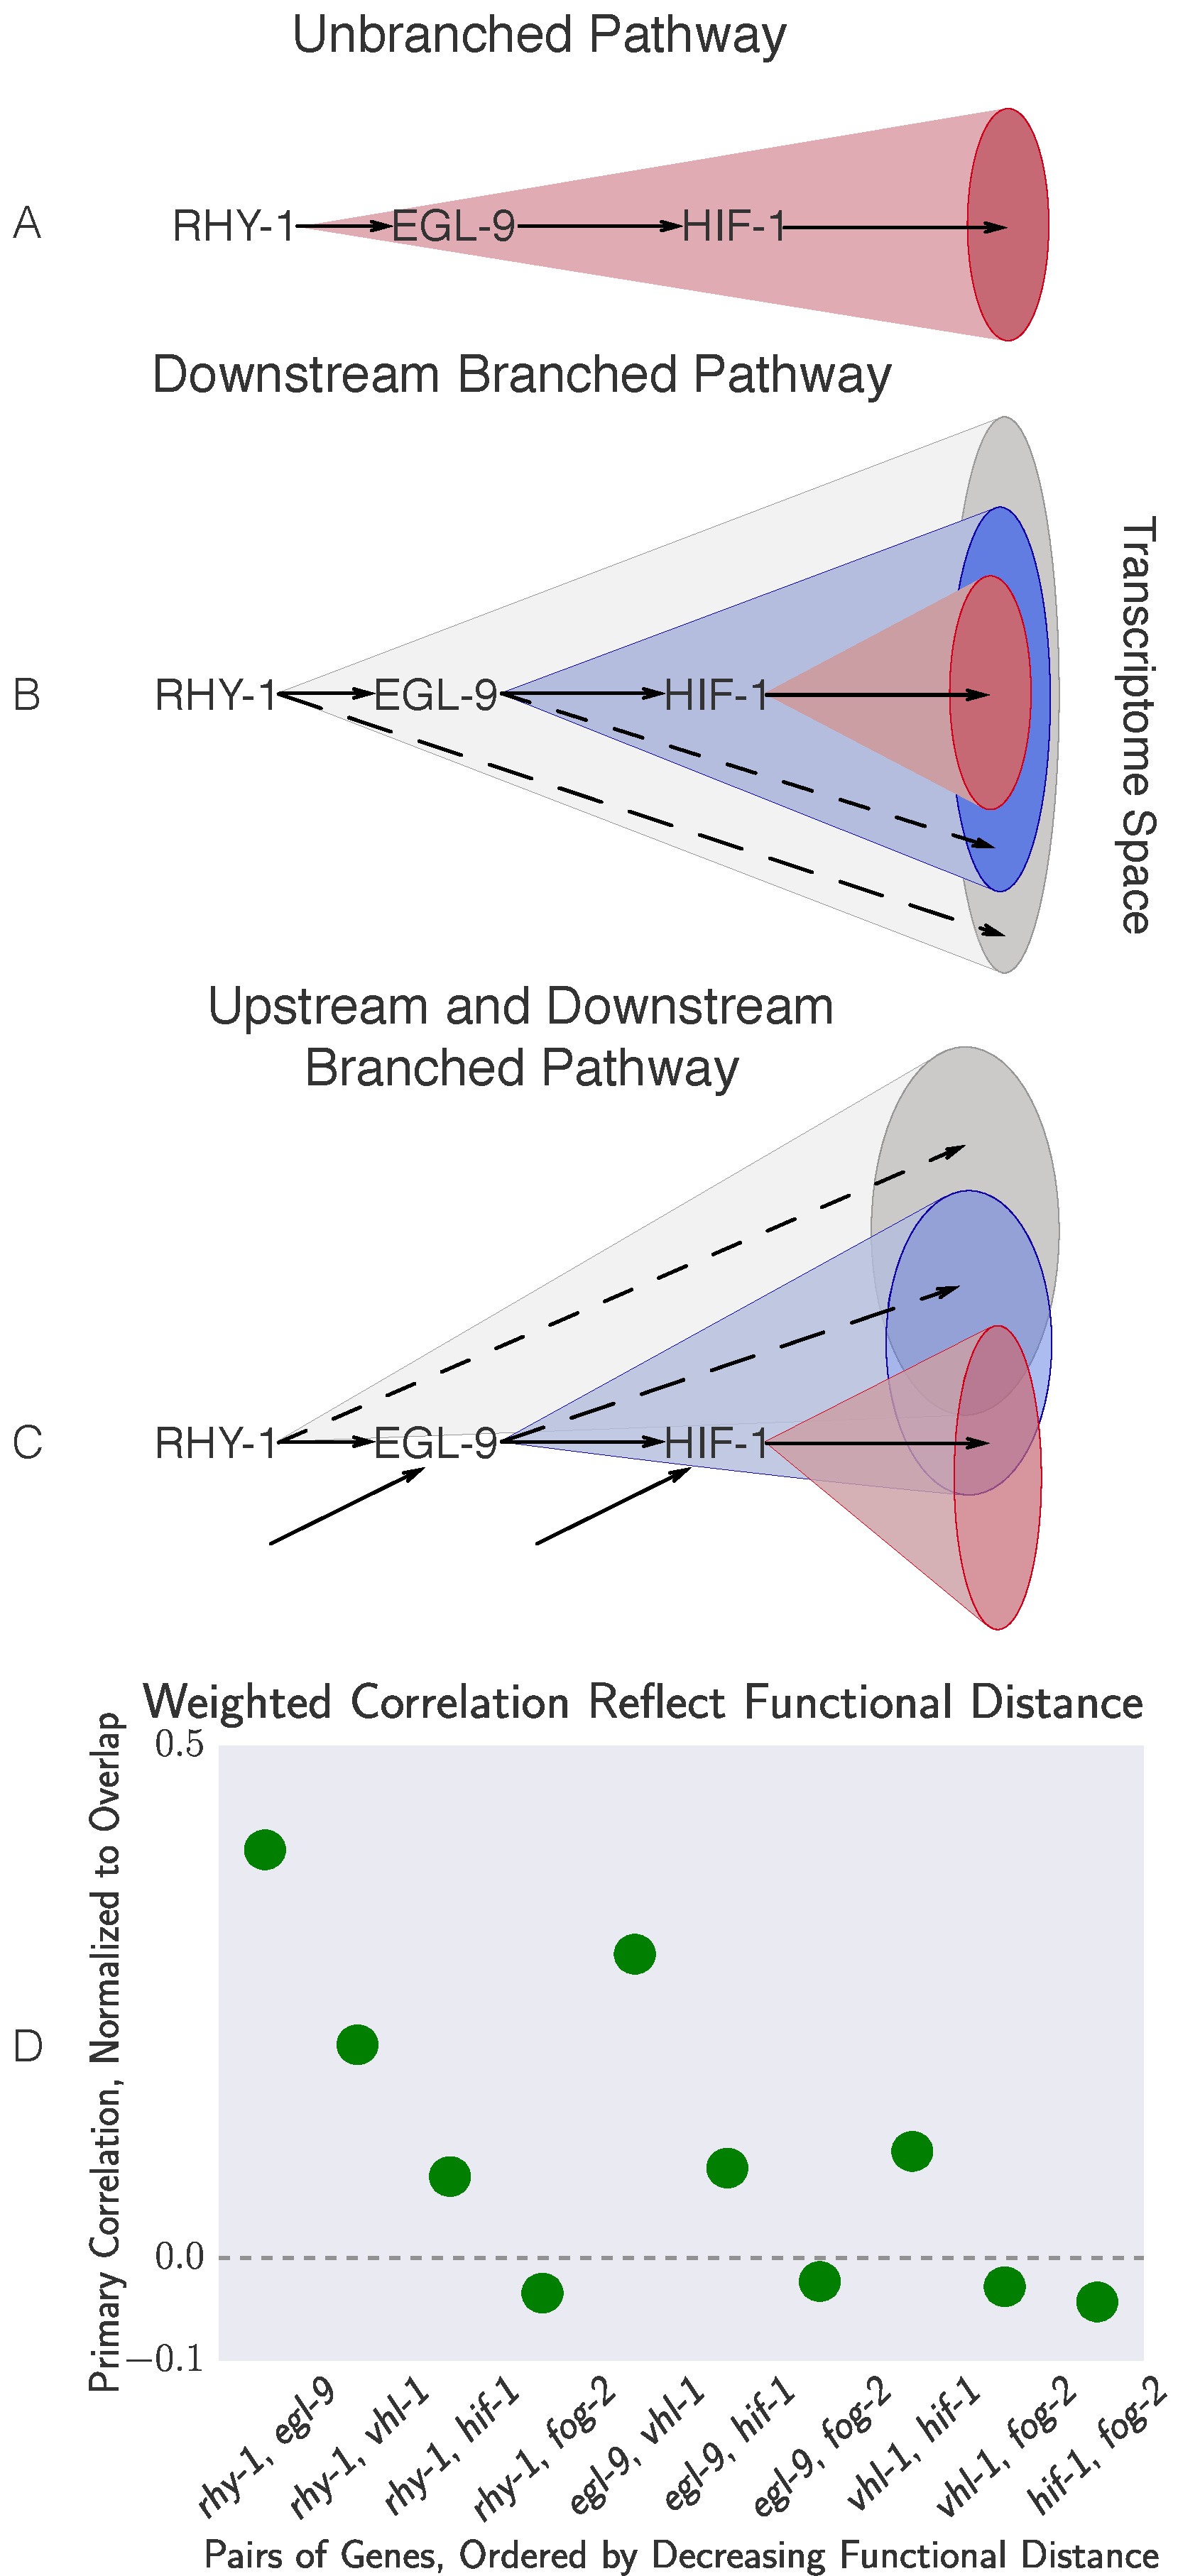
\includegraphics[width=\linewidth]{figs/decorrelation.pdf}
\caption{
Theoretically, transcriptomes can be used to order genes in a pathway under certain assumptions. Arrows in the diagrams above are intended to show the direction of flow, and do not indicate valence.
\textbf{A} A linear pathway in which \rhy{} is the only gene controlling \egl{}, which in turn controls \hif{} does not contain transcriptomes with enough information to infer the order between genes.
\textbf{B} On the other hand, if \rhy{} and \egl{} have transcriptomic effects that are separable from \hif{}, then the \rhy{} transcriptome should contain contributions from \egl{}, \hif{} and \egl{}- and \hif{}-independent pathways. This pathway contains enough information to infer order.
\textbf{C} If a pathway is branched in both upstream and downstream directions, observed transcriptomes will show even faster decorrelation. Nodes that are separated by many edges may begin to behave almost independently of each other with marginal transcriptomic overlap or correlation, reflecting the weak control distant nodes exert on each other.
\textbf{D} The hypoxia pathway can be ordered according to functional distance. The rapid decay in correlation is probably due to a mixture of upstream and downstream branching that happens along this pathway.
% Top: Pairwise weighted correlations between transcriptomes can be used to infer functional distance between interacting genetic partners. Pairwise correlations are ordered by increasing network distance between genes. Correlations were weighted by the fraction of genes that overlapped between the two genes being compared. Notice that correlations involving the \fog{} negative control are very near zero. Error bars represent standard deviation of the weighted correlation. Bottom: Simplified schematic of the hypoxia pathway shown to illustrate functional distance between genes in the pathway.
}
\label{fig:decorrelation}
\end{figure}

We investigated the possibility that transcriptomic signals do in fact contain relevant information about the degrees of separation by weighting the robust bayesian regression of each pairwise analysis by $N_\mathrm{Overlap}/N_{\mathrm{detected}}$. We plotted the weighted correlation of each gene pair, ordered by increasing functional distance (see Fig.~\ref{fig:decorrelation}). In every case, we see that the weighted correlation decreases monotonically due mainly, but not exclusively, to decreasing $N_\mathrm{Overlap}$.
We believe that this result is not due to random noise or insufficiently deep sequencing. Instead, we propose a framework in which every gene is regulated by multiple different molecular species, which induces progressive decorrelation.
This decorrelation in turn has two consequences. First, decorrelation within a pathway implies that two nodes may be almost independent of each other if the functional distance between them is large. Second, it may be possible to use decorrelation dynamics to infer gene order in a pathway, as we have done with the hypoxia pathway\footnote{An important question is whether a looped circuit like the hypoxia pathway can be ordered in the way we have ordered it in Fig.~\ref{fig:decorrelation} since a loop does not technically have a beginning. One explanation is that we studied the hypoxia pathway under normoxic conditions, and therefore the control of \hif{} over \rhy{} and \egl{} is weak, effectively turning the looped pathway into a linear one. Probably, under hypoxic conditions the pathway would effectively be reversed.
}.

\subsection{Identification of novel targets and biological processes in the hypoxia response}
\label{sub:new_biology}
% TODO: Add SI folder information
So far, our analysis has focused mainly on extracting genetic relationships between the set of mutants we sequenced. Our dataset also provides us with a unique view of the \hif{}-dependent response in \cel{}. In total, we identified \total{} differentially expressed genes that are altered in any of the hypoxia pathway mutants. Of these \total{} genes, \inall{} genes were differentially expressed in all the hypoxia mutants. Because of the extensive feedback between \hif{} and \egl{}, we expected to identify a small subset of genes that were up-regulated or down-regulated consistently in every hypoxia mutant except the \egl{};\hif{} double mutant.
We identified \allup{} genes that were up-regulated in this manner, and \alldown{} genes that were down-regulated (see SI for gene identities). These genes likely constitute a core response around the circuit in question, and their behaviour should reflect the genetic relationships the best. Indeed, graphing these genes shows beautiful agreement with predictions (see \url{www.wormlabcaltech.github.io/mprsq} for interactive graphics).

% TODO: Citation needed at end of paragraph?
In order to identify affected biological processes, we performed an in-house gene ontology enrichment analysis using annotations provided by WormBase, followng the procedure shown in TEA~\cite{Angeles-Albores2016}. Top enriched terms included `hydrolase activity' (869 observed hits; 7.8 fold change; p-value $<10^{-10}$); `organic anion transport' (803 hits; 7.5; p-value $<10^{-10}$); `spliceosomal complex' (647 hits; 8.2 p-value $<10^{-10}$); `SAM-depdendent methyltransferase activity' (1215 hits; 6.6; p-value $<10^{-10}$); and `cell division' (1251 hits; 7.9; p-value $<10^{-10}$).
In mammals, the mammalian target of rapamycin pathway (mTOR), which is intimately associated with the hypoxia pathway, has been previously linked to osmotic stress responses~\cite{Zhou2007}. Our findings also suggest that the \hif{}-dependent response causes important changes in chromatin structure via activation or recruitment of chromatin remodelling factors, as well as changes in isoform processing.

% TODO: Citations needed
We identified downstream targets of the genes we studied that were not associated with other genes in the \hif{} circuit. \vhl{} targets were particularly easy to isolate because \vhl{} does not seem to participate in the \rhy{}, \egl{}, \hif{} feedback circuit, and as a result it is easy to isolate targets for that are \hif{}-independent. We found \vhltargets{} genes downstream of \vhl{}. These \vhltargets{} genes include \emph{pole-1}, an ortholog of human polymerase $\epsilon$ catalytic subunit; \emph{F33H2.6}, an ortholog of the human regulator of microtubule dynamics 1 (RMDN1)\cite{}; and many solute carriers.
Reflecting this, enriched GO terms were `ion binding', `growth', `cell division', `cell projection assembly' as well as `ion binding' and `divalent metal ion transport'. \vhl{} has been previously implicated as a controller of mitotic fidelity in renal cell carcinoma~\cite{Hell2014}. Our findings support a role of \vhl{} in chromosomal integrity and mitotic fidelity. Furthermore, recent reports suggest that solute carriers may be associated with poor prognosis in clear-cell renal carcinoma~\cite{Liu2015}, which highlights the biological relevance of our predictions.

% TODO: SI link
We identified \hiftargets{} genes that are activated by \hifp{}. We verified that the genes we identified are actually \hif{} targets by searching for a set of 20 gold-standard genes from the literature~\cite{Shen2006,Shen2005} in our gene set, and found that \hif{} targets were significantly enriched in these genes ($p<10^{-7}$). GO term enrichment indicated that this list was associated with `cell division', `SAM methyltransferase activity' and `cellular modified amino acid metabolic processes'. A full list of \hif{} targets can be found in S.I..

\subsection{Discovery of New Pathways: \nog{}}
\label{sub:nog1}

% TODO: Expand on this opener
Enzymes rarely have a single substrate. Although the role of \egl{} in \hif{} hydroxylation has been clearly elucidated, the roles of \hif{}-independent \egl{} effects remain largely unknown and had not been explored until relatively recently~\cite{}. Using our experimental design, we were able to measure transcriptomic epistasis in our double mutant. A corollary of measuring epistasis is that we can now identify genes that violate the epistasis relationships between the genes we studied. As a particular example, we focused on a gene called \nog{}.

% nog1
\begin{table}%[tbhp]
\centering
\caption{Using \nog{} as a genetic reporter reconstructs a new pathway and identifies \nog{} downstream to \egl{}.}
\begin{tabular}{llrrr}
Single Mutant & Double Mutant & $\beta_\mathrm{single}$ & $\beta_\mathrm{double}$ \\
\midrule
1. \egl{} & \egl{};\vhl{} & $6.10$ & $6.23$\\
2. \vhl{} & \egl{};\vhl{} & $6.45$ & $6.23$\\
3. \egl{} & \egl{};\hif{} & $6.08$ & $6.02$\\
4. \hif{} & \egl{};\hif{} & $3.56$ & $6.02$\\
\bottomrule
\end{tabular}

\addtabletext{Our genetics design allows us to identify genes that don't agree with the model we have built.
\nog{} appears to be under strong control by \egl{} and \vhl{}, probably through hydroxylation and ubiquitination of an unknown factor that drives transcription to \hif{}. \nog{} is not a target of \hif{}, since \hif{} loss of function has a weaker effect than \egl{} and the \egl{};\hif{} double mutant shows the same expression level as \egl{}.}
\label{tab:nog1}
\end{table}



\section*{Discussion}

\subsection{The Hypoxia Circuit in \cel{}}

% new model:
\begin{figure}[tbhp]
\centering
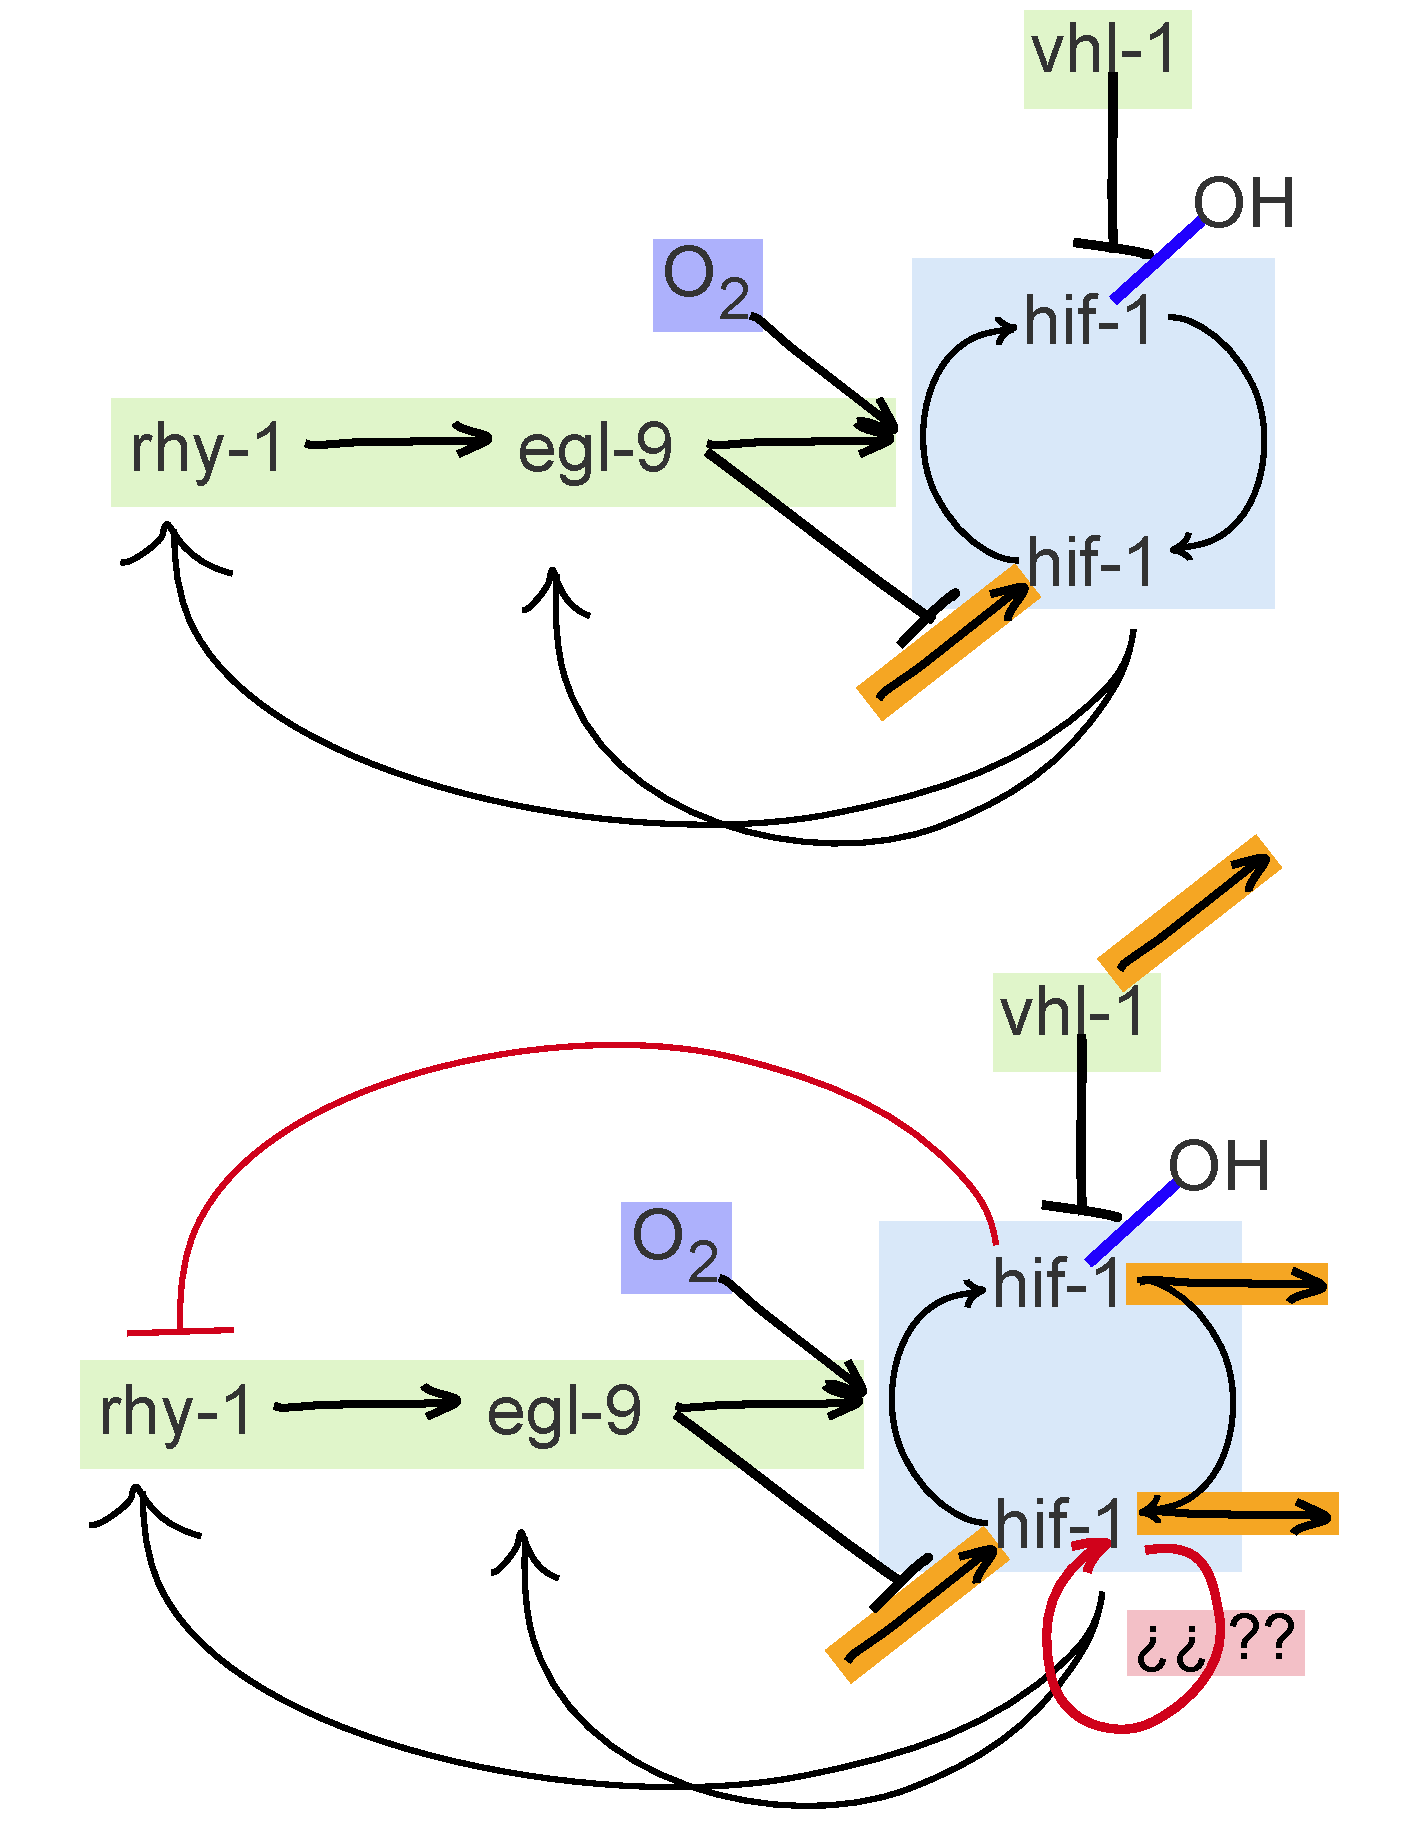
\includegraphics[width=\linewidth]{figs/new_model.pdf}
\caption{A schematic of the hypoxia pathway in \cel{}. \rhyp{} likely inhibits a protein-protein interaction between \eglp{} and CYSL-1~\cite{Ma2012}. This interaction inhibits the activity of \eglp{}. When active, \eglp{} can inhibit \hifp{} by catalyzing the hydroxylation of \hifp{}, which leads to its recognition and ubiquitination by \vhlp{} and ultimately leads to rapid degradation of \hifp{} protein. Independently of its enzymatic function, \eglp{} can also inhibit \hifp{} transcriptional activity. Our results identified \rhy{}, \egl{} and \cysl{} as downstream targets of the \hif{}-dependent transcriptional response.
However, we also identified increased in the mRNA levels of \rhy{} and \cysl{} when \hif{} was knocked out.
Moreover, the \hif{} knock-out transcriptome correlated positively with \rhy{}, \egl{} and \vhl{}. One plausible explanation for these observations is that hydroxylated \hifp{} has transcriptional consequences.
Inset shows a simplified diagram of the hypoxia pathway.
}
\label{fig:newmodel}
\end{figure}

Previous work has established a circuit in which \rhy{} activates \egl{} in a linear pathway, and \egl{} inhibits \hif{} in an oxygen-dependent manner. Hydroxylated \hifp{} can then be degraded in a \vhl{}-dependent manner. There is also evidence that \egl{} and \rhy{} are in turn activated by \hif{}~\cite{Bishop2004,Powell-Coffman2010}.
Finally, there is evidence that although the interaction between \egl{} and \vhl{} is important for \hif{} repression, \egl{} can also act in a non-\vhl{} dependent manner (see Fig.~\ref{fig:newmodel} top).

We were able to impute the positive regulatory relationship between \egl{} and \rhy{}. We would not have been able to infer the order of the regulation without additional information. Using clustering as a proxy for phenotype, we were able to infer the relationship between \egl{} and \hif{}. We were also able to infer a positive (linear or AND) relationship between \egl{} and \vhl{} using clustering. Alternatively, we gained the same information by performing \emph{in silico} qPCR on the genes under study. \emph{In silico} qPCR also revealed that \hif{} has two states with different activities: Non-hydroxylated \hifp{} increases levels of \rhy{}, and hydroxylated \hifp{} inhibits \rhy{} and possibly \egl{} as well, although the double mutant did not recapitulate that interaction. We also revealed that \hif{} is an autoregulator.

These discoveries are consistent with a homeostatic circuit. By autoregulating itself, \hif{} can mantain appropriate protein levels both in normoxic and hypoxic conditions. Inhibition of \rhy{}, and possibly of \egl{}, ensures that an appropriate equilibrium is maintained between hydroxylated and non-hydroxylated protein, which may have functional consequences for the cell if both forms are active.

In addition to these biological findings, our dataset allows us to generate predictions of genes that may be under direct \hif{} regulation. Assuming that non-hydroxylated \hifp{} has different activities from hydroxylated \hifp{}, we identified 5 genes that are candidates for activation by hydroxylated \hifp{}. These genes have been implicated in the \cel{} immune response, or have behavioural phenotypes, underscoring the importance of \hif{} in neurobiology and immunology~\cite{Gray2004,Cheung2005,Chang2008,Ma2013}.

\subsection{Towards A Genetic Theory of Transcriptomics}
We have shown that transcriptomes contain sufficient information to be used as semi-quantitative phenotypes in metazoans. These phenotypes can be interpreted globally via correlation tests, clustering or other probabilistic methods; alternatively, they can be used to query single reporter genes in a manner similar to qPCR today. Transcriptomic phenotypes have distinct advantages over physical traits.
Firstly, due to their increased complexity, the genotype-phenotype mapping degeneracy ought to be greatly reduced, which facilitates predictions of genetic interaction. Secondly, genes that result in subtle or no visible traits when mutated may have strong (detectable), reproducible phenotypes at the transcriptomic level, which would make the study of small-effect genes significantly easier.

RNA-Seq and microarray datasets have been used previously by bioinformaticians to generate high-throughput predictions of genetic interactions and consortiums such as the The Cancer Genome Atlas have sequenced RNA from many different cancers in the hope of identifying clinically or biologically relevant interactions~\cite{}. By correlating many different datasets in many different conditions, it is possible in theory to predict genetic interaction. Our approach differs from these high-throughput methods in that we are not attempting to generate large scale networks. Rather, the strength in our analysis derives from our experimental design, which allows us to ask and answer a large number of questions about the functional interactions between genes.
As a by-product, we are also able to identify genes related to the core circuit studied in question, but our main goal is not to generate databases or predict large numbers of interactions between a large number of genes. We have shown that transcriptomic phenotypes can capture distinct interaction modes in a single experiment, making it possible to infer complex regulatory relationships between genes. By measuring these transcriptomes under a rigorous experimental design, it is possible to identify many relationships simultaneously. With the advent of fast pseudo-alignment tools and ever cheaper sequencing techniques, biologists should consider using global transcriptomes as a tool beyond hypothesis generation or target acquisition.
We have developed a genetic framework to deal with sequence-based phenotypes. Here, we have shown that global transcriptomes can be readily dealt with under this framework. In the future, we hope that other sequence-based phenotypes will shed new insights into genetic relationships between genes.


\matmethods{
\label{methods}
\subsection*{RNA-Seq}
Tagmentation etc

We used Kallisto to perform pseudo-read alignment and performed differential analysis using Sleuth. We fit a generalized linear model for a transcript $t$ in sample $i$:
\begin{equation}
  y_{t,i} = \beta_{t, 0} + \beta_{t, genotype}\cdot{}X_{t, i} + \beta_{t, batch}\cdot{}Y_{t, i} + \epsilon_{t, i}
\end{equation}

where $y_{t, i}$ are the logarithm transformed counts; $\beta_{t, genotype}$ and $\beta_{t, batch}$ are parameters of the model, and which can be interpreted as biased estimators of the log-fold change; $X_{t, i}, Y_{t, i}$ are indicator variables describing the conditions of the sample; and $\epsilon_{t, i}$ is the noise associated with a particular measurement.

\subsection*{Genetic Analysis}
Genetic analysis of the processed data was performed in Python 3.5. Our scripts made extensive use of the Pandas, Matplotlib, Scipy, Seaborn, Sklearn, Networkx, Bokeh, PyMC3, and TEA libraries~\cite{Team2014,McKinney2011,Oliphant2007,Pedregosa2012,Salvatier2015,VanDerWalt2011,Developers,Angeles-Albores2016,Waskom}.
Our analysis is available in a Jupyter Notebook~\cite{Perez2007}. All code and required data (except the raw reads) are available at \url{https://github.com/WormLabCaltech/mprsq} along with version-control information. Our Jupyter Notebook and interactive graphs for this project can be found at \url{https://wormlabcaltech.github.io/mprsq/}. Raw reads were deposited at XXXXXXXXXXX}

\showmatmethods{}% Display the Materials and Methods section

\acknow{This article was written with support of the Howard Hughes Medical Institute.}

\showacknow{} % Display the acknowledgments section

% \pnasbreak splits and balances the columns before the references.
% If you see unexpected formatting errors, try commenting out this line
% as it can run into problems with floats and footnotes on the final page.
% \pnasbreak{}

% Bibliography
\bibliography{citations}

\end{document}
